\section{The utility of dynamic HPFC in snake robot locomotion}

Most of the snake robot locomotion strategies today are intended for flat surfaces. Lateral undulation and sidewinding are two of these strategies presented in \ref{subsec:traditional-loco}. Even though they are based on flat surfaces, they require some amount of ground friction to yield propulsion. Either way, the snake robot body motions are the basis for the propulsion. A position controller for the joint angles of the snake robot would thus induce a satisfying behavior. Consequently, a hybrid position/force controller would simply be an overkill for these strategies. The concertina locomotion strategy, on the other hand, is conducted in narrow spaces where the snake robot anchors itself against the environment. This is also explained further in \ref{subsec:traditional-loco}. A joint controller is sufficient in this case as well if one only considers the curling up and stretching out of the robot. It might however be desired for the snake robot to push against its environment at the same time as this movement takes place. A hybrid position force controller could then be useful to simultaneously realize these control goals.

Compliance control, presented in \ref{subsec:compliance-control}, is another control option for adapting to the environment. The main difference between compliance control and dynamic HPFC is that the compliance controller is a so called reactive controller, meaning that the robot will change its curvature according to the environment when a contact feedback has been received. The dynamic HPFC contrarily uses a feedforward term for dynamic force, enabling it to always control both the force and position precisely. The success of this method does to a large degree depend on a correct modeling of the dynamics of the robot and its environment.

The locomotion method which can take the most advantage of the dynamic HPFC is the OAL method presented in \ref{subsec:OAL}. The possibility to control position and force simultaneously and independently in different directions allows the snake robot to both move between obstacles and push against them at the same time. Furthermore, the dynamical control facilitates a dynamical or compliant, rather than stiff, behavior. This is beneficial for the mechanical parts of the snake robot which can then experience a lower level of strain and wear and tear. 


%Give a brief overview of the most important strategies for terrestrial snake robot locomotion, and discuss the prospective properties of HPFC in the context of your findings.

%- Controlling both the force and position using compliance control would require us to frequently switch between very very high and very low compliance. Det er vel directional compliance tho

%- vi likevel ha en viss compliant behavior i at hvis en hindring beveger seg litt vil slangen følge etter --> men det kan være en assumption at hindringene har statisk posisjon

%- posisjonsstyring gir stiv oppførsel og krafstyring gir dynamisk oppførsel

%%%%%%%%%%%%%%%%%%%%%%%%%%%%%%%%%%%%%%%%%%%%%%%%%%%%%%%%%%%%%%%%%%%%%%%%%%%%%%%%%%%%%%%%%%%%%
%%%%%%%%%%%%%%%%%%%%%%%%%%%%%%%%%%%%%%%%%%%%%%%%%%%%%%%%%%%%%%%%%%%%%%%%%%%%%%%%%%%%%%%%%%%%%
%%%%%%%%%%%%%%%%%%%%%%%%%%%%%%%%%%%%%%%%%%%%%%%%%%%%%%%%%%%%%%%%%%%%%%%%%%%%%%%%%%%%%%%%%%%%%

\section{Application challenges related to dynamic HPFC}

There are surely several ways of implementing and designing the dynamic HPFC control logic on a snake robot. This section will focus on the challenges related to the application of the suggested design scheme in \ref{subsec:DHPFC}. Special attention is paid to the chosen variable spaces and the consequences of configuration transitions when the snake robot moves.

\subsection{Computational challenges}

Whenever the snake robot achieves successful forward or backward propulsion it will slide along the obstacles that are by its side. Eventually the contact between a given link and an obstacle will be lost. At this point, the obstacle will either be left alone or come in contact with a neighboring link. These two scenarios are illustrated in Figures \ref{fig:obst_slide_seq1} and \ref{fig:obst_slide_seq2} respectively. If the contact is completely lost, it means that one constraint is lost as well and $n_c = n_c - 1$. This will in turn lead to the variable $\mathbf{r}_t$, describing the position of the contacts, shrinking. Consequently the mapping matrix $\mathbf{E}$ to the allowed force and movement directions will shrink as well. The greatest challenge in this case is changing the dimensions of the affected variables in real time. One option could be keeping all variable spaces unchanged and instead set the parts of $\mathbf{E}$ corresponding to the lost constraint to zero so that it has no impact on the following solution.

\begin{figure}[h!]
    \centering
    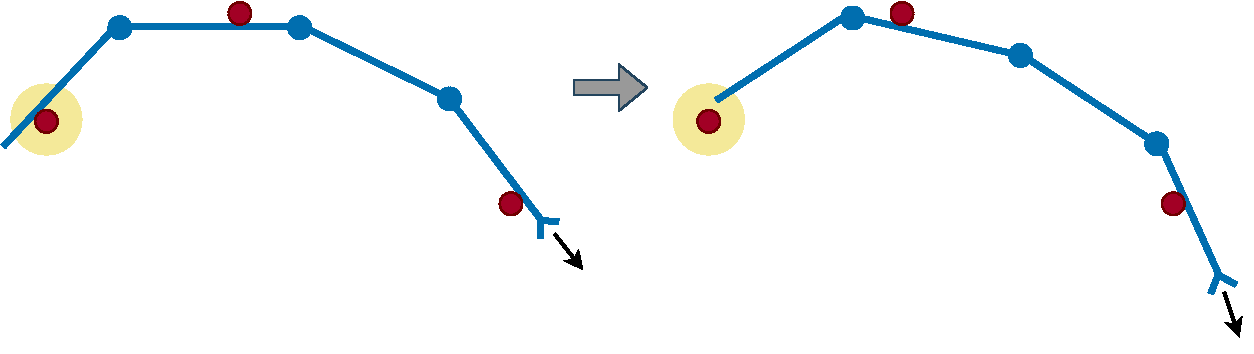
\includegraphics[width=\textwidth]{figures/theory/obst_slide_sequence1.pdf}
    \caption{Snake robot losing contact with obstacle}
    \label{fig:obst_slide_seq1}
\end{figure}

\begin{figure}[h!]
    \centering
    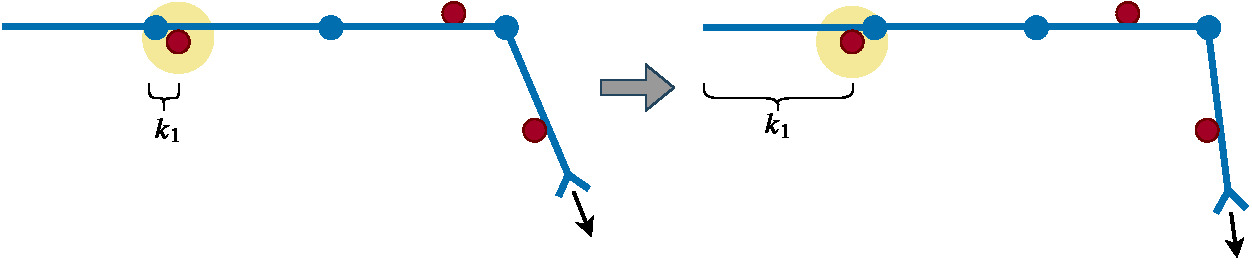
\includegraphics[width=\textwidth]{figures/theory/obst_slide_sequence2.pdf}
    \caption{Obstacle changing contact from one link to another}
    \label{fig:obst_slide_seq2}
\end{figure}

If, on the other hand, the snake simply slides in a way that the contact is transferred to an adjoining link, the size $n_c$ and dimensions of all variables will remain unchanged. In addition to this, the obstacle will lie on the same side of the snake as it already was, which enables the direction of the desired force application to the obstacle to stay the same. Thus, the constraint will generally be on the same form. The only thing that has to change is the description of the position variables in $\mathbf{r}_t$ belonging to the new contact point. Again, the change is most probably slim since the two first variables $(x_t, y_t)$ describe the position of the contact point and the obstacle is assumed to be static (meaning its position will not change even though the calculation of the position changes). Furthermore, the adjoining link adopting the contact is probable to have a similar angle $\theta_t$ relative to the base frame as the previous link given that the desired path is well designed and defined. From this it follows that the joint variable $\phi_c$ back to the obstacle frame will stay similar to what it was as well. These aspects obviously make the implementation simpler and the control sequence smoother and more predictable.

Even though the numerical value of the mentioned variables do not change drastically, the Jacobian will have to be recalculated since the variables now are described by a new subset of the joint variables. Finding a new expression for the Jacobian matrix and its derivative in real time is not a trivial, nor fast, operation. One option would of course be pre-computing $\mathbf{J}$ and $\dot{\mathbf{J}}$ for every link that could be in contact with an obstacle and only employ the ones that are relevant at the specific time instance. There is however still a challenge related to this case. The generalized joint variables $\mathbf{q}$ contain the distances $k$ from the contact points to the preceding joints. It is important that these distances are not mixed and that they are only used once. In other words, two contact points should not be described by the same $k$. As a consequence of this, the Jacobian for every link would have to be computed with all the possible $k$'s. Logically, this would in turn lead to a large number of pre-computed matrices as the number of links and obstacles grow. In addition to this, the right set of Jacobians would have to be chosen real time while administering that they all use unique $k$'s. This should be done without changing the existing setup more than necessary in order to avoid jumps in the control. It is very much an achievable task, but at the same time an extra challenge.

With a contact moving from one link to another, the corresponding joint variable $k$ describing the position of the contact point will change and the manner in which it is computed will also change. This is once again an achievable, yet challenging task to perform in real-time. It should also be noted that the value of this $k$ will probably experience a jump. This is because the contact moves from the end of a link to the beginning of a link, or vice versa, and the distance is always measured with respect to the preceding joint of the link in contact. This is illustrated in Figure \ref{fig:obst_slide_seq2}. On the other hand, it is reassuring that the matrices $\mathbf{M(q)}$ and $\mathbf{C(q,\dot{q})}$ are unaltered by the change of a $k$. This is logical since these matrices describe the dynamics of the snake robot alone.

The greatest challenge arises if the number of contact points increase. This means that the dimension of all variables will have to increase correspondingly and the Jacobians have to be either re-computed or re-assembled. It is in this case important to keep in mind the challenge associated with memory allocation in the software being used.

\subsection{Differences with the traditional manipulator case}

One significant challenge related to snake robots as opposed to traditional robot manipulators is the presence of passive joints at the base of the robot. The passive joints of the snake robot that are attached to the base frame, $[\phi_0, x_0, y_0]$ are included in the description of the position of every link and contact point. This means that if they were actuated, they could have influenced all the points that are desired to control, given that the robot is not stuck between obstacles. The dynamic hybrid position/force controller could therefore introduce a desired joint acceleration value $\ddot{\mathbf{q}}_d$ for these passive joints when recalculating from the desired contact point accelerations $\ddot{\mathbf{r}}_{t,d}$. Since these joints are passive, they are also uncontrollable and a desired control input on the joints is not realizable. A greater number of joints will generally make this challenge more insignificant because it leads to a larger degree of controllability of all contact points.

When it comes to the assignments of traditional robot manipulators and snake robots, they are usually a lot more repetitive and pre-defined for robot manipulators. A typical task for an industrial hybrid position force controlled robot manipulator is polishing a known surface with a given pressure. An example is given in Figure \ref{fig:robotman-polish}. The snake robot might also be familiar with the shape of its current environment, but this is something that is constantly changing as the robot moves through the world. Thus, the position and force application requirements are constantly changing as well. Furthermore, since the snake robot is eventually meant to locomote through outdoor environments, it will encounter different kinds of obstacles as illustrated in Figure \ref{fig:weird-env}. They can differ in both size, texture and be either soft or rigid. Thus, there are a lot of factors the snake robot will have to take into account. For this project however, the environment and control goals are significantly simplified.

\begin{figure}
    \centering
    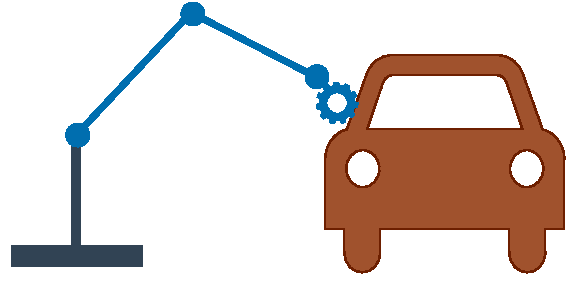
\includegraphics[width=0.6\textwidth]{figures/theory/robotman-polish.pdf}
    \caption{Industrial robot manipulator polishing a car}
    \label{fig:robotman-polish}
\end{figure}

\begin{figure}
    \centering
    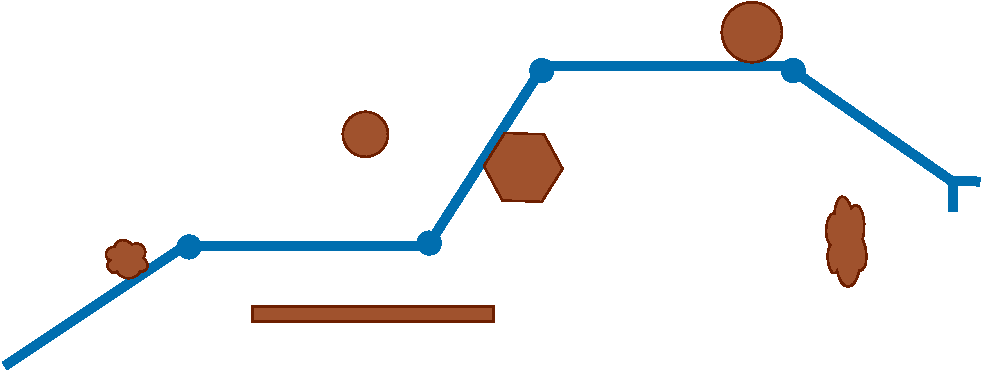
\includegraphics[width=0.7\textwidth]{figures/theory/weird-environment.pdf}
    \caption{Snake robot in environment with varying obstacle types}
    \label{fig:weird-env}
\end{figure}

There is also a considerable difference in the typical constraints on a snake robot and a traditional manipulator. Manipulators usually only have constraints or obstacles in the close environment of the end effector in which the manipulator is performing a task. It might also have some limitations regarding the motion span of its joints, but this applies to snake robots as well, though perhaps to a smaller degree. The environment the snake robot is traversing may as mentioned contain various and spread out obstacles, making the constraints different from time to time. If, however, a robot is in an undesirable position between obstacles, a snake robot might have an advantage in that it can exit its current configuration from several different directions since no part of it is fixed to any point in the world.

%- Arbitrary number of obstacles and constantly changing requirements (desired force application etc, as opposed to a typical industrial manipulator that simply should polish a surface with a given pressure repeatedly)

%- The environment is constantly changing and the contact wont be a point contact in the real world, and the snake robot might encounter all kinds of surfaces and textures (rigid, soft, slippery etc)